\section{Implementierung von Mimikry}
In diesem Kapitel werden die technischen Implementierungsaspekte der aktuellen Mimikry Architektur beschrieben. Die Diagramme modellieren wichtigere Komponente der hier angewandten Model-View-Presenter (MVP) Architektur und die Zusammenhänge zwischen den Komponenten. Die Variablen, Funktionen und Methoden (siehe Appendix: Allgemeine Konzepte der Programmierung) innerhalb der Diagramme bilden die MVP spezifische Logik ab. 
Dieses Entwurfsmuster trennt die Verwaltung der Daten mittels einer Datenschicht aus der Model Komponente von der Steuerungslogik der graphischen Oberfläche der View Komponente. Die beiden Klassen Kommunizieren mit Hilfe eines Mediators, dem sog. Presenter~\cite{mvc}. MVP wurde von der bekannten Model View Controller (MVC) Architektur abgeleitet~\cite{Sok.214}, die in der vorherigen Version implementiert und nachträglich zu der MVP Struktur umgebaute wurde. Die Struktur von den Einführung und Feedback Screens (Siehe Kapitel 3, Konzeption) wird hier nicht abgebildet. Schließlich erfolgt die Beschreibung der Implementierung einer lokalen Datenbank.

\subsection{Architektur des Mimikry Modul - MVP}
Die Architektur des Mimikry Moduls ist eine androidspezifische Architektur, \\Model- View-Presenter. In der MVP Architektur ist die Model Komponente für die Verwaltung von Daten zuständig. Die View Komponente manipuliert die graphische Oberfläche und sollte möglichst wenig Logik beinhalten. Die Steuerungslogik befindet sich in der Presenter Komponente, die mit den View und Model Komponenten verbunden ist. Das Model und die View sind nicht direkt miteinander verbunden und daher übernimmt der Presenter die Kommunikation. Durch die Trennung der Klassen vom Android-SDK lässt sich der selbst gestalteter, nicht androidspezifischer Code separat Testen, was den Entwicklungsprozess optimiert. Siehe Abb.\ref{architekture}. 
Das Mimikry Modul beinhaltet drei Hauptaktivitäten, siehe Abb. \ref{mimicrystructure}. Jede der Aktivitäten: MimicryActivity, MimicryPreviewActivity, MimicryNoPreviewActivity wird als eine separate View Komponente angesehen. Jede der Views schafft Grundlagen für eine separate View-Presenter-Struktur, im Unterschied zum Model, das von mehreren Klassen geteilt wird. 
Die Architektur der zu der MimicryActivity zugehörigen Struktur wird als ein durchgängiges Beispiel beschrieben, die Unterklassen MimicryPreviewActivity, MimicryNoPreviewActivity wurden nach dem gleichen Prinzip gebaut.

\begin{figure}
    \centering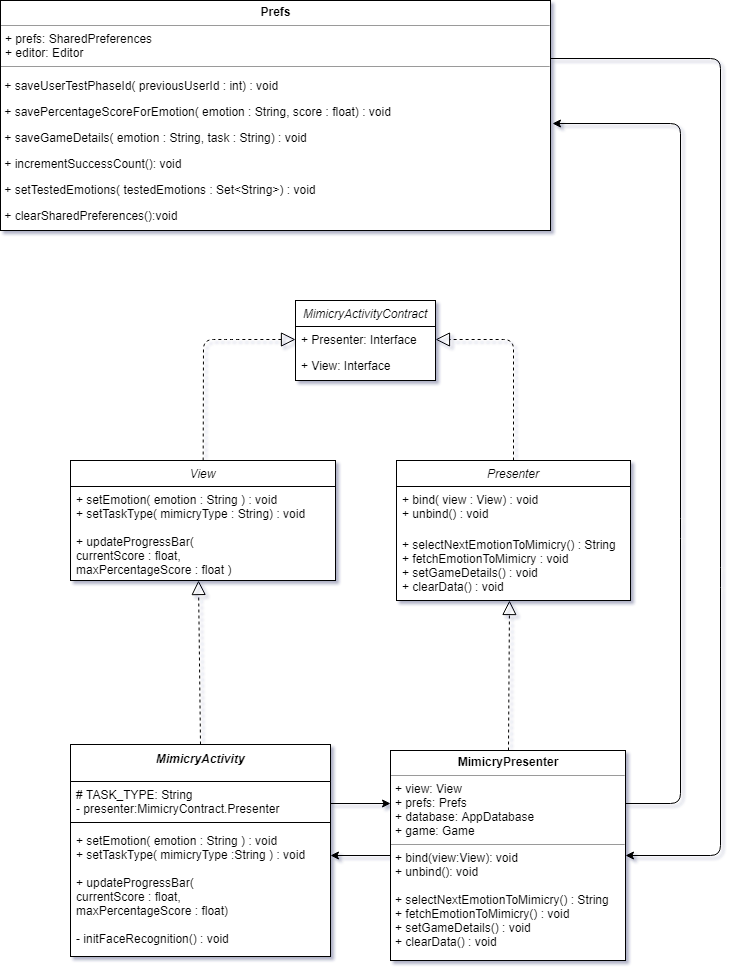
\includegraphics[width=390pt]{res/mvp_final.png}
\caption{Die beiden View und Presenter Interfaces befinden sich innerhalb eines MimicryActivityContract Interfaces. Für MimicryPreviewActivity und MimicryNoPreviewActivity Varianten werden außer separaten Presenter Klassen auch separate Contract Klassen implementiert.}
\label{architekture}
\end{figure}

%Da Software Entwicklung für mobile Geräte ein dynamischer Prozess ist, werden abhängig von der Größe und des Ziel des Projektes verschiedene Lösungsansätze optimal~\cite{mvc}.
%Da die App keine aktive Internetverbindung und sonstigen externen Informationen benötigt, war die Model Komponente weniger relevant als bei anderen typischen Beispielen der MVP Architektur. 
\subsubsection{Model}
Das Model des Mimikry Moduls ist die Prefs Klasse vgl. Abb.\ref{architekture}. Die Prefs Klasse ist für die Verwaltung von Daten zuständig. Bei Projekten mit einem anderen Fokus würden sich hier externe Interaktionen wie Netzwerkanfragen oder Datenbank API Anfragen befinden. Mimikry speichert einige von SHORE\re abgefangenen Daten in SharedPreferences. Daher wurde die Logik für das Speichern und Aktualisieren von Daten in SharedPreferences innerhalb der Klasse Prefs gruppiert.

Die Beschreibung der Methode getEmotionToMimicry:
Die Methode getEmotionToMimicry wird (von dem Presenter) aufgerufen. Sie liefert als Rückgabewert eine Zielemotion die im String Format aus der Daten des nächsten Spiels in den SharedPreferences abgelesen und zurückgegeben wird.
Falls das Ablesen der Daten nicht gelungen wäre, würde ein Ersatzstring zurückgegeben werden um einen NullPointerException zu vermeiden. 
\begin{minted}{java}
    public String getEmotionToMimicry() {
        return prefs.getString(EMOTION, DEFAULT);
    } 
\end{minted}
\newpage
\subsubsection{View}
Die  View Komponente besteht aus MimicryActivity und einem innerhalb der Activity erzeugten CameraPreviewFragment. 

Die Klasse CameraPreviewFragment vgl. Abb.\ref{view}, die an der Fraunhofer Institut entwickelt und im Rahmen dieser Bachelorarbeit erweitert wurde, befindet sich innerhalb der MimicryActivity. Sie gehört also zu der View Komponente. Dieses Fragment ist eine Anzeige, die für Gesichtserkennung, Messen der Emotionsausrücke und ihre Übergabe an MimicryActivity mittels einen CallbackScoreListener zuständig ist. Der aktuelle Wert wird an den Presenter weitergeleitet und in einer lokalen Datenbank gespeichert.\\

\begin{figure}[!ht]
    \centering\includegraphics[width=220pt]{res/CameraPreviewFragment.png}
\caption{CameraPreviewFragment aus SHORE\re wurde erweitert. Es wurde unter anderem eine Struktur für die Übergabe von Daten mittels einem CallbackListener implementiert.}
\label{view}
\end{figure}
\newpage
Nach der Interaktion von dem Benutzer, also einer Imitation eines Gesichtsausdrucks wird ein Prozess der Übergabe der Daten an die MimicryActivity mit einem Aufruf der Methode \\sendScoreObject initiiert, vgl. den Code darunter. Da es sich um das Neusetzen eines Wertes auf dem Fortschrittsbalken handelt, wurde der Callback auf dem Hauptthread, dem sogennanten UI Thread ausgeführt. Folgender Code ist für diesen Prozess zuständig. Der Callback benachrichtigt die MimicryActivity, innerhalb welcher sich das CameraPreviewFragment befindet.
\begin{minted}{java}
 private void sendScoreObject(float happyScore,
                              float sadScore,
                              float angryScore,
                              float surprisedScore) {
        final MimicryScore scoreObject = new MimicryScore(happyScore,
                                                          sadScore, 
                                                          angryScore,
                                                          surprisedScore);
        getActivity().runOnUiThread(new Runnable() {

            @Override
            public void run() {

                scoreListener.updateScore(scoreObject);
            }
        });
    }
\end{minted}
\newpage
Die abstrakte Klasse MimicryActivity, siehe Abb. \ref{mimicrystructure} ist eine Oberklasse für MimicryPreviewActivity und MimicryNoPreviewActivity. Es wurden zwei Interfaces: CallbackScoreListener und MimicryContract.View implementiert, siehe Abb.\ref{mimicrystructure}.
Nach dem Callback von dem CallbackScoreListener benachrichtigt MimicryActivity den Presenter und übermittelt die Daten.

Beschreibung von dem Code, der den Presenter benchrichtigt:
Das Presenter Objekt innerhalb der Klasse MimicryActivity (View Komponente, Abb.\ref{mimicrystructure}, Abb.\ref{architekture}) ruft Methoden aus dem Presenter Interface auf. Dadurch kommuniziert Der Presenter mit dem Model.
\begin{minted}{java}
    presenter.setGameDetails();
    presenter.fetchEmotionToMimicry();
    presenter.fetchTaskType();
\end{minted}

MimicryActivity reagiert auch auf die vom Presenter auf View aufgerufenen Methoden und verändert ihre graphische Oberfläche. Die Klasse beinhaltet auch eine Methode initFaceRecognition, die das CameraPreviewFragment erzeugt, die für die Aufnahme des Benutzers und den Emotionserkennungsprozess zuständig ist. Die View Komponente bleibt unabhängig von der Model Komponente.
\begin{figure}[!ht]
    \centering\includegraphics[width=330pt]{res/mimicry_activity_structure_final.png}
\caption{Die hierarchische Struktur der View Komponenten: abstrakte Klasse MimicryActivity mit einem zugehörigen ScoreListener Interface und zwei spezialisierte Unterklassen, MimicryPreviewActivity und MimicryNoPreviewActivity. Jede der Klassen ist mit einem View Interface verbunden, der alle für die Presenter Komponente verfügbaren Methoden beinhaltet. }
\label{mimicrystructure}
\end{figure}

In den Unterklassen der MimicryActivity(MimicryPreview und MimicryNoPreview), siehe \ref{mimicrystructure}, die die View-Komponenten darstellen, werden je nach dem Aufgabetyp die graphischen Elemente angepasst. Es wird auch ein ein Zeitbalken iniitiert. Beide Mimicry Akitivitäten unterscheiden sich, weil es so gemäß dem Design vorgesehen wurde. Sie beinhalten aber auch viele Schnittstellen, daher und wegen der Codekohärenz mit dem restlichen Teil der App wurde die Vererbung mit der abstrakten Klasse MimicryActivity vorgesehen.
In der MimicryPreviewActivity werden vier TextViews mit Grundemotionen angezeigt. Sobald die Zielemotion gewählt wird, wird eine der TextViews mittels der setActiveEmotionLabel Methode, siehe \ref{mimicrystructure} hervorgehoben.
In der MimicryNoPreviewActivity wird zusätzlich ein Layout für die Vermittlung der Zielemotion separat von dem Imitieren (Nachahmen) implementiert. Das Layout für das Ankündigen der Emotion wird für 10 Sekunden angezeigt. Danach wird es ausgeblendet und ein Layout für das eigentliche Spiel wird eingeblendet. Der Name ''NoPreview'' bezieht sich auf Mängel einer Vorschau der Aufnahme. Stattdessen wird innerhalb der Fläche die Zielemotion als Text angezeigt. 
\newpage
\subsubsection{Presenter}
Die Presenter Komponente ist ein Mediator zwischen der View und Model Komponente. Der Presenter beinhaltet die Steuerungslogik der visuellen Komponente, je nach dem aktuellen Zustand des Models.

\begin{figure}[!ht]
    \centering\includegraphics[width=200pt]{res/presenter.png}
\caption{Presenter Komponente beinhaltet ein spezialisiertes View Objekt, das mit den Methoden bind und unbind an die View Komponente gebunden wird. Auf diesem View wird vom Presenter die Methode updateEmotionLabel aufgerufen, die eine Rückmeldung des Presenters in dem MVP Verlauf abbildet.}
\label{presenter}
\end{figure}

Die Umsetzung von dem Presenter erfolgte mit der MimicryPresenter Klasse, vgl.\ref{architekture} die von keiner Android spezifischen Klasse erbt. MimicryPreviewPresenter und MimicryNoPreview Presenter wurden ebenso für die jeweiligen spezialisierten Unterklassen implementiert. Die Presenter Klassen implementieren MimicryContract. Presenter Interface, der alle von den Presenter verfügbaren Methoden beinhaltet. 
MimicryPresenter Komponente reagiert auf ankommenden Daten, speichert, aktualisiert oder lädt diese mittels der Prefs Klasse, also dem Model (siehe den Code darunter) und benachrichtigt das View.

Beschreibung der Methode fetchEmotionToMimicry:
Nach dem Aufruf von dem Presenter Objekt aus MimicryActivity wird unter anderem die Methode fetchEmotionToMimicry aufgerufen. Danach erfolgt die Überprüfung auf null, um den in Java bekannten NullPointerException zu vermeiden. Sobald es gesichert wurde, dass das View existiert, wird das Objekt der Prefs Klasse (Model) benachrichtigt. Die Zielemotion im Textformat wird dann aus dem Model als ein Parameter der Methode setEmotion von View vermittelt. Das View wird darauf entsprechend reagieren und die graphische Oberfläche anpassen. Dadurch kommuniziert der Presenter mit dem Model. Das Model kommuniziert zurück und liefert neue Daten dem Presenter und der Presenter benachrichtigt das View.
\begin{minted}{java}
    public void fetchEmotionToMimicry() {
        if (view == null){
            return;
        }
        view.setEmotion(prefs.getEmotionToMimicry());
    }
\end{minted}
\subsubsection{Ablauf der Mimikry MVP Architektur}
Die Einführung der MVP Struktur dient der Verbesserung der Übersichtlichkeit und Trennung der Logik für die Tests, die außerhalb des Android Geltungsbereichs durchgeführt werden messen. 
Sobald ein neues Messergebnis in dem CameraPreviewFragment entsteht, wird die MimicryActivity durch ein Callback von dem CallbackScoreListener aus dem CameraPreviewFragment benachrichtigt. Der aktuelle Wert wird von der Activity aus dem Presenter vermittelt und durch den Presenter in der lokalen Datenbank und in den SharedPreferences gespeichert. Als eine Rückmeldung benachrichtigt der Presenter die View, vgl.\ref{architekture}, um den Fortschrittsbalken mit einem aktuellen Ergebnis zu aktualisieren. 
Das Speichern der Werte in SharedPreferences wurde mittels der Prefs Klasse implementiert, um eine schnelle Auswertung, das Speichern und Ablesen der höchsten erreichten Werte zu ermöglichen. Die Werte, die in der Datenbank gespeichert werden, werden ausschließlich für den Zweck der Studie gespeichert. Beides erfolgt innerhalb der Logik des Presenter.
Der Presenter wird als ein Objekt in der MimicryActivity erzeugt und mit Methoden bind und unbind an den Lifecycle als den Lebsnzyklus der Activity gebunden. Die Methode fetchEmotionToMimikry kommuniziert mit dem Prefs Model und liest die Werte ab, die in SharedPreferences gespeichert wurden. Die Methode clearData leert alle Spiel spezifischen Werte. Das Speichern in der lokalen Datenbank erfolgt mit der setGameDetails Methode.

\subsection{Einbindung von Shore\re}
Sentinel\_LDK und ShoreJavaWrapper sind externe Pakete, die für den Zweck der Realisierung der Aufgabenstellung von dieser Bachelorarbeit von Frauenhofer Institut zur Verfügung gestellt wurden für akademische, nicht kommerzielle Zwecke gestattet. Der Gebrauch der Software wird durch die Boost, Lua und Lua Plus Lizenzen bestimmt~\cite{shore},~\cite{Kueblbeck}.

\subsection{Die lokale Datenbank für die Studienphase}
Um die Ergebnisse, die während der Studie ausgewertet werden zu speichern, wurde eine Implementierung der MySQLite Datenabank mit Hilfe von der Bibliothek Room umgesetzt.
Room ist eine Abstraktionschicht für MySQLite und ermöglicht einen einfachen Zugang und Interkation mit den Daten~\cite{Room}. Um die gesammelten Daten zu sehen, wurde das Android-Debug-Database Tool benutzt~\cite{ADD}. Die Daten wurden als Game Objekte gespeichert. Für das Speichern der komplexen Objekte wurde eine Klasse Converter eingeführt, die Daten für ein ganzes Spiel in dem JSON Format Speichert. Ein Game Objekt besteht aus einer ID von dem Benutzer, einer ID von dem Spiel, Typ des Spiels und die zu jeweiligen Emotionen passenden Messwerten, die als Arrays für einzelne Emotionen gespeichert wurden.
Die Ergebnisse können auch einen Wunsch für wissenschaftliche Zwecke vermittelt werden.
